\chapter[Planificación]{
  \label{chp:plan}
  Planificación e avaliación de custos
}
\minitoc
\newpage

Neste capítulo explicarase a planificación do traballo realizado e a avaliación de custos. 

\section{Concepción do proxecto}

Como xa se comentou na sección \ref{orixe}, o proxecto nace dun \textbf{encontro con membros de radios comunitarias}. Naquel mesmo momento obtivéronse unha serie de primitivas historias de usuario, máis centradas entón na redifusión e a organización que na escoita. A seguinte lista é unha \textbf{transcrición das notas tomadas} durante ese encontro:

\begin{itemize}
	\item Os usuarios dos sistema son as propias emisoras.
	\item As emisoras teñen que poder engadir audios.
	\item As emisoras poden acceder aos audios das outras.
	\item As emisoras teñen que poder saber quen está a emitir os seus programas.
\end{itemize}

Cómpre clarificar que o listado anterior só se trata de impresións que, finalmente, inspiraron este traballo. En \textbf{modo algún se deben tomar coma obxectivos do proxecto}, pois estes non foron definidos até a primeira reunión ou iteración 0 (ver sección \ref{it0})

\section{Iteracións}

Como se explicou no capítulo \ref{chp:metodoloxia} a cerca da metodoloxía, o desenvolvemento executouse de  de forma \textbf{iterativa e incremental}. Unha iteración consiste nun ciclo de desenvolvemento cuns obxectivos a cumprir (historias de usuario) e unha reunión co cliente onde se fai unha valoración dos progresos e se recollen novas historias de usuario.

Ao ser isto un proxecto de final de carreira, contaranse coma reunións co cliente as sesións de \textbf{revisión de progresos} entre o director do proxecto e o alumno. Estas reunións tiveron unha periodicidade quincenal (aproximadamente, dependendo da dispoñibilidade)


\subsection{Primeira reunión (Iteración 0)}
\label{it0}

Na primeira reunión estableceuse a \textbf{lista de obxectivos xerais do proxecto} repasados xa no listado da sección \ref{obxectivos}. Estes supoñen unha aproximación ao problema máis ambiciosa que a idea orixinal de ter un simple directorio web compartido entre emisoras pois ten en conta as \textbf{necesidades dos ouvintes} e a propiedade dos programas por parte dos seus autores e non necesariamente da emisora, cousa bastante común no mundo da radio comunitaria. Foi neste momento cando se tomou a decisión de utilizar \textbf{Django} coma framework de desenvolvemento e \textbf{PostgreSQL} coma sistema de xestión de bases de datos.

Os obxectivos de cara a primeira iteración foron:

\begin{itemize}
	\item Facer un primeiro borrador do deseño do \textbf{modelo de datos}.
	\item Investigar a manipulación de \textbf{ficheiros RSS} utilizando Python. Desde o principio, a consulta dos ficheiros de RSS intuíuse coma o xeito de manter actualizados os programas mais neste momento aínda non se tomara unha decisión firme de como facelo.
\end{itemize}

\subsection{Iteración 1}

Cumpríronse os obxectivos marcados, entregando un \textbf{deseño preliminar do modelo de datos} na data estimada (figura \ref{fig:classold}) 

\begin{figure}[h]
	\centering
	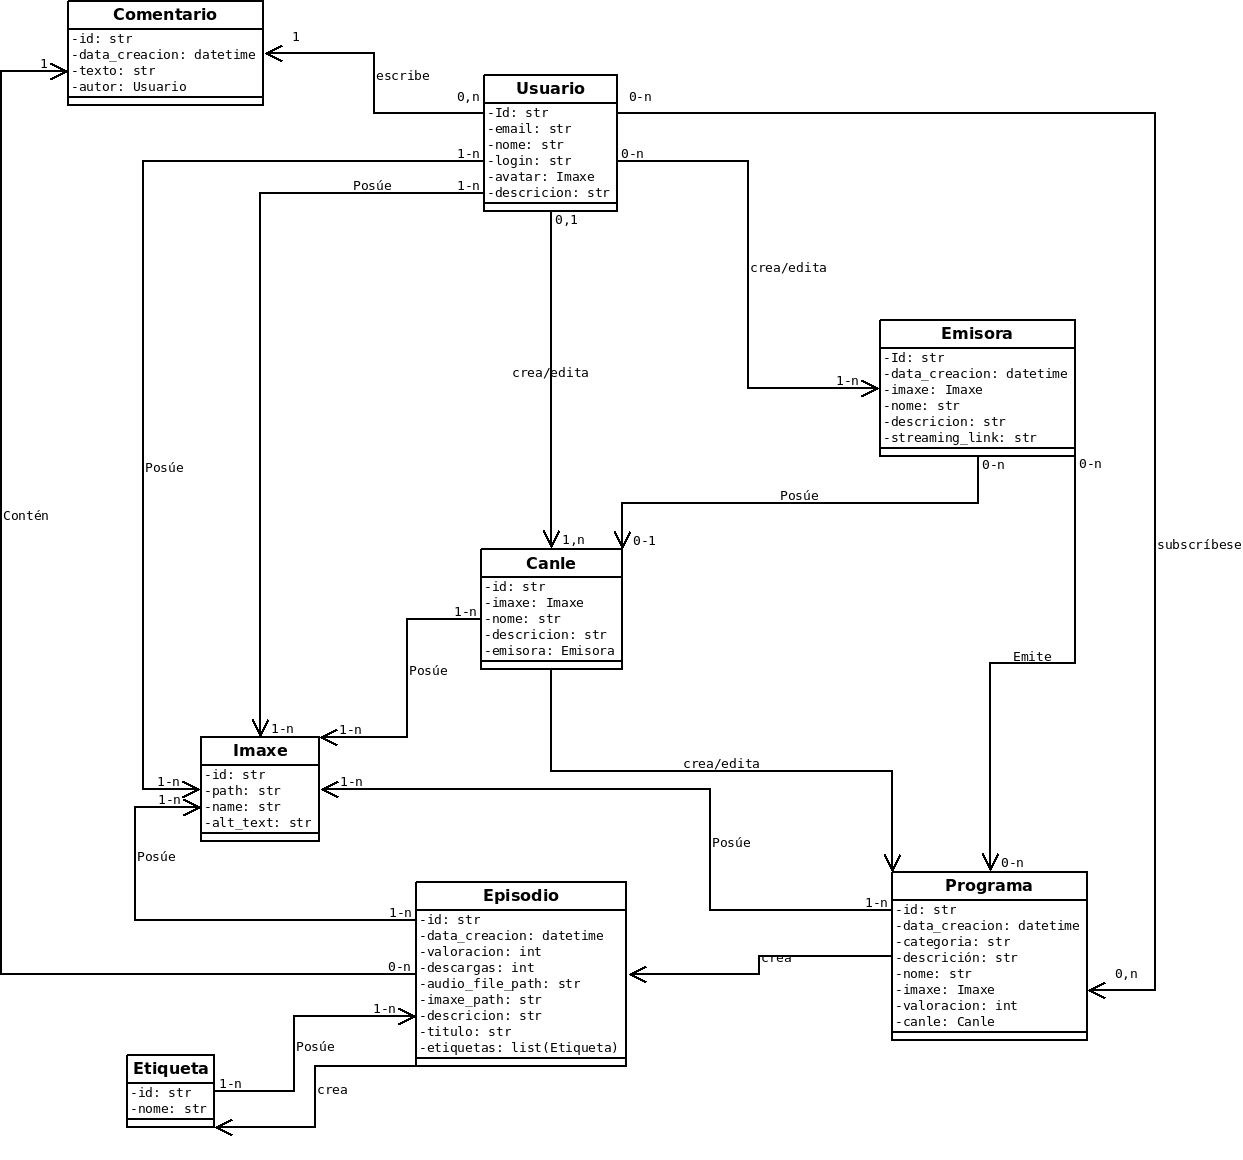
\includegraphics[scale=0.35,keepaspectratio=true]{./images/class_diagram_20171107.png}
	\caption{It1: Diagrama de clases do primeiro borrador de deseño.}
	\label{fig:classold}
\end{figure}

Unha cousa a comentar neste primeiro modelo é a existencia dunha clase \textbf{\say{canle}} intermediaria entre a emisora e o programa que, como veremos, quedou finalmente desbotada. A idea era que os colectivos que realmente teñen unha emisión por onda e aqueles que publican podcasts de escoita baixo demanda terían necesidades distintas e debían diferenciarse, sempre sen bloquear a posibilidade de que unha radio emitise podcasts.

En canto ao RSS, fixéronse os primeiros \textbf{scripts de lectura}. Ese primeiro código era capaz de descargar un ficheiro RSS e transformalo nun obxecto cos datos do programa que á súa vez contiña unha lista de obxectos cos datos dos episodios, demostrando que a consulta de RSS si era a forma axeitada de afrontar a inserción e actualización dos contidos.

Novos obxectivos:

\begin{itemize}
	\item \textbf{Instalar a infraestrutura} desenvolvemento: Instalación do entorno Django-PostgreSQL.
	\item Implementación de \textbf{Programa e Episodio}.
	\item Implementación dunha \textbf{interface web básica}.
	\item Ampliar o código do \textbf{script de lectura} dos ficheiros RSS.
\end{itemize}

\subsection{Iteración 2}

Configurouse o entorno de Django e as ferramentas de desenvolvemento. Utilizouse a \textbf{técnica TDD} (ver capítulo \ref{chp:metodoloxia} sobre a metodoloxía) as clases Program e Episode coas súas correspondentes táboas nunha base de datos controlada mediante \textbf{PostgreSQL}. Esas primeiras clases aínda non contiñan información das imaxes nin das etiquetas e os datos non extraíbles do RSS contiñan valores nulos. O sistema executábase sobre o \textbf{servidor de desenvolvemento} de Django, algo que se mantivo durante todo o proceso de desenvolvemento por comodidade e eficiencia. Creouse tamén un repositorio para o \textbf{control de versións} utilizando a plataforma GitHub (ver sección \ref{git})

Conseguiuse a medias o obxectivo de servir unha interface web sinxela: Amosábanse os datos gardados, pero non servía para engadir novo contido aínda. Desprazouse ese obxectivo á seguinte iteración.

\begin{figure}[h]
	\centering
	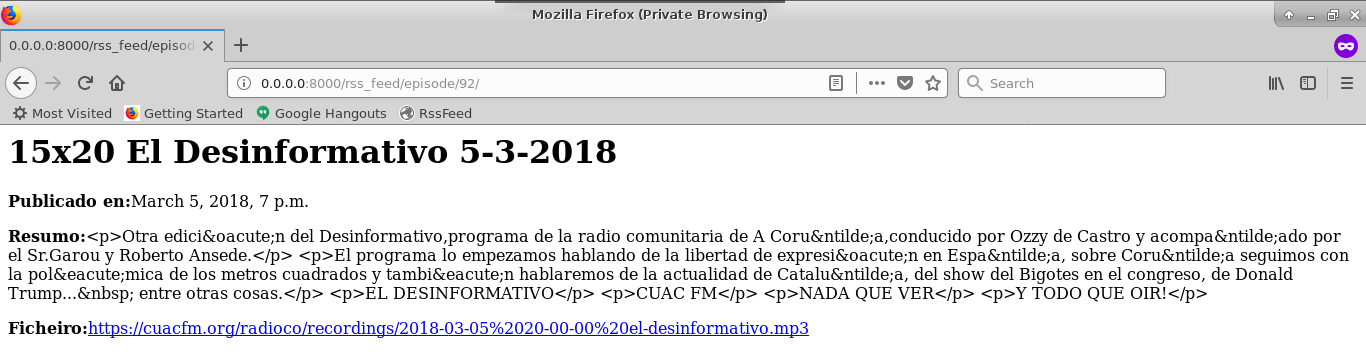
\includegraphics[scale=0.3,keepaspectratio=true]{./images/it2_episode.png}
	\caption{It2: Interface web. Páxina dun episodio.}
	\label{fig:it2_episode}
\end{figure}

Os traballos de ampliación do código de lectura de RSS leváronse a cabo: Os programas e episodios recollían toda a información requirida no momento agás á de imaxe e de etiqueta (tag). Os traballos neste código revelaron a necesidade de dispor de \textbf{distintos tipos de lector} dependendo da fonte da que o ficheiro RSS fose extraído. 

Cos obxectivos de instalación e configuración cumpridos, comezou a recompilación de historias de usuario: 

\begin{itemize}
	\item Engadir \textbf{formularios} á interface para crear novos programas desde ela.
	\item Implementar \textbf{novos tipos de lector} de RSS.
	\item Aplicar \say{plantillas} de \textbf{estilos} ao frontend. 
\end{itemize}

\subsection{Iteración 3}

Creouse o formulario de envío do enlace RSS. Instalouse o soporte de Django para \textbf{Bootstrap 4}, podendo así usar eses modelos. Utilizándoos, creouse unha páxina de engadir programa co aspecto amosado na figura \ref{fig:it3_add_program}.

\begin{figure}[h]
	\centering
	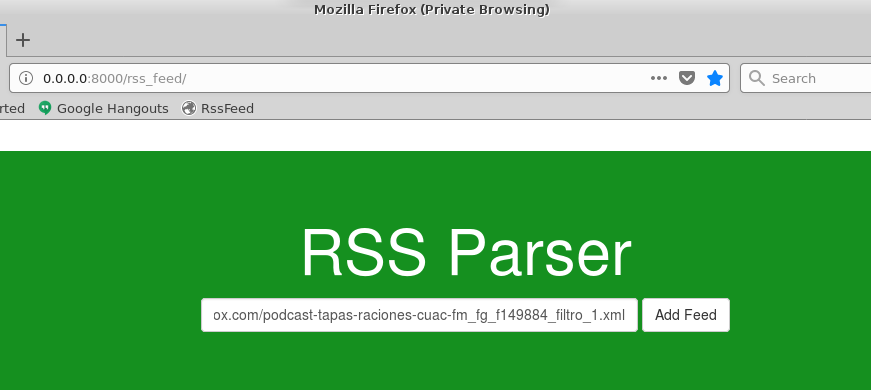
\includegraphics[scale=0.5,keepaspectratio=true]{./images/it3_add_program.png}
	\caption{It3: Interface web. Páxina de engadir programa.}
	\label{fig:it3_add_program}
\end{figure}

Implementouse o soporte para os distintos formatos de ficheiro RSS: Ao principio da iteración só se podían engadir ficheiros extraidos de \textbf{RadioCo}. Ao final, os parsers para \textbf{Ivoox e Podomatic} quedaron tamén implementados. Pese a que os 3 funcionaban, a calidade do código non era a satisfactoria.

Novas historias de usuario:

\begin{itemize}
	\item \textbf{Refactorización} dos lectores de RSS.
	\item Implementación das clases de \textbf{imaxe e etiqueta}.
	\item Redefinir a \textbf{estrutura} das páxinas. 
\end{itemize}


\subsection{Iteración 4}

Nesta iteración créase un \textbf{módulo específico} para as funcións de lectura de RSS. Aplícase un \textbf{patrón estratexia} para dar soporte a distintos parsers cunha interface única (máis detalles no capítulo \ref{chp:disenho} sobre o deseño). Para completar o proceso de inserción de programas e episodios, implementáronse as clases da imaxe e etiqueta (Image e Tag).

\begin{figure}[h]
	\centering
	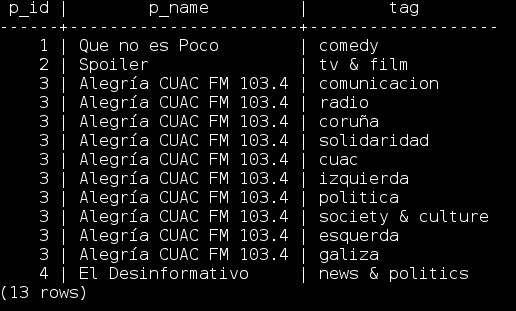
\includegraphics[scale=0.6,keepaspectratio=true]{./images/tags.png}
	\caption{It4: Resultado de consulta á base de datos relacionando programas cos seus tags.}
	\label{fig:it4_tag}
\end{figure}

No tocante á interface, introducíronse nesta iteración as follas de estilo con \textbf{CSS-Grid}, definindo un deseño que serviu coma base do que máis tarde sería o deseño definitivo.

Novos obxectivos:

\begin{itemize}
	\item Crear un proceso que corra no servidor para \textbf{manter os programas actualizados}.
	\item Engadir \textbf{usuarios} ao sistema. 
\end{itemize}

\subsection{Iteración 5}

Levouse a cabo a instalación de \textbf{Celery} e as súas dependencias para correr procesos sobre os seus fíos. Reutilizouse o código do módulo que contén os parsers de RSS. 

No tocante aos usuarios, escribiuse unha primeira versión da \textbf{autenticación} e o rexistro, o cal deu pé a relacionar os usuarios cos seus programas engadidos. Porén, a clase usuario por defecto de Django non satisfacía as necesidades previstas.

Novas historias de usuario:

\begin{itemize}
	\item Estender a clase Usuario.
	\item Crear páxina de edición de Ususario.
	\item Facer as vistas dependentes da autenticación.
\end{itemize}

\subsection{Iteración 6}

Introduciuse unha \textbf{clase de apoio} para outorgarlle ao usuario de Django unha serie de atributos necesarios no sistema. Introduciuse a comprobación de autenticación naquelas vistas que o requirisen, por exemplo, engadir programa, como se ve nas figuras \ref{fig:it6_log} e \ref{fig:it6_anon}.

Fíxose unha primeira implementación da vista de \textbf{edición de usuario}, pero sen soporte para o cambio de contrasinal. Quedaría para a iteración seguinte.

\begin{figure}[h]
	\centering
	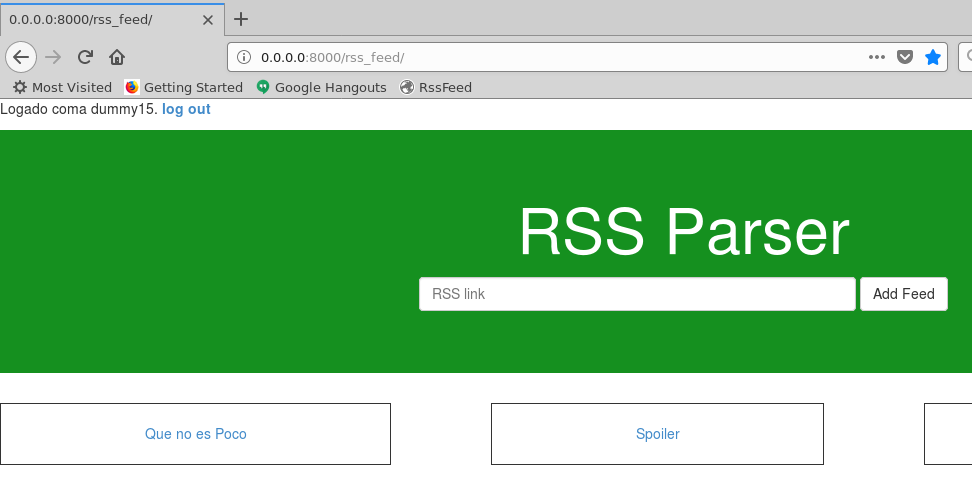
\includegraphics[scale=0.4,keepaspectratio=true]{./images/it6_log.png}
	\caption{It6: index.html para usuario identificado.}
	\label{fig:it6_log}
\end{figure}

\begin{figure}[h]
	\centering
	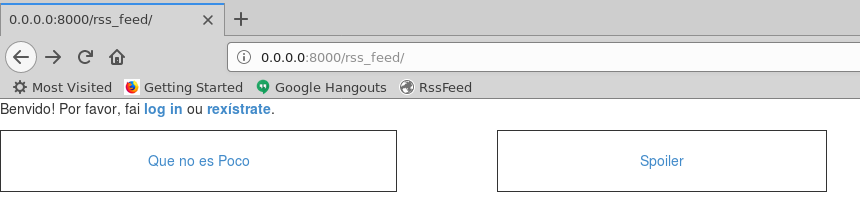
\includegraphics[scale=0.5,keepaspectratio=true]{./images/it6_anon.png}
	\caption{It6: index.html para usuario anónimo.}
	\label{fig:it6_anon}
\end{figure}

Novas historias de usuario:
\begin{itemize}
	\item Completar páxina de \textbf{edición de usuario}.
	\item Implementar clases para os \textbf{votos e os comentarios} dos episodios.
	\item Implentar a clase de \textbf{emisora e canle}.
	\item Crear \textbf{deseño de interacción} das páxinas.
\end{itemize}

\subsection{Iteración 7}

Debuxáronse uns \textbf{deseños esquemáticos} das distintas páxinas de \textbf{interface web} e definiuse a navegación entre elas. Este deseño de interface foi xa o definitivo. Valería, en diante, coma guía para confeccionar as distintas vistas. Poden verse algúns borradores no capítulo \ref{chp:disenho} sobre o deseño.

O resto de obxectivos foron cumpridos. Nesta iteración decidiu \textbf{desbotarse a clase de Canle} por ter unhas funcións moi limitadas e solaparse en gran parte con Emisora.

Novas historias de usuario:
\begin{itemize}
	\item Dar soporte á \textbf{internacionalización}.
	\item Crear vista para engadir \textbf{novas emisoras}.
\end{itemize}


\subsection{Iteración 8}

Engadiuse o soporte de Django para a internacionalización e fíxose unha primeira \textbf{tradución} da web a lingua galega. Non obstante, o seu \textbf{funcionamento non era o axeitado}. Dado que se estaba empregar moito tempo nesta tarefa sen acadar ningún resultado, decidiuse pospoñela.

Co gallo de situar o selector de idioma, fíxose unha \textbf{cabeceira} para situar as ferramentas transversais ás vistas.

Integráronse a vista de engadir programa e a nova de crear emisora nunha única, chamada \say{engadir contido}. Debido ao bloqueo sufrido pola tarefa de internacionalización, sobrou tempo que se empregou en implementar a vista da páxina principal (index) e a vista de detalles de emisora (figura \ref{fig:station_detail_final}).

\begin{figure}[H]
	\centering
	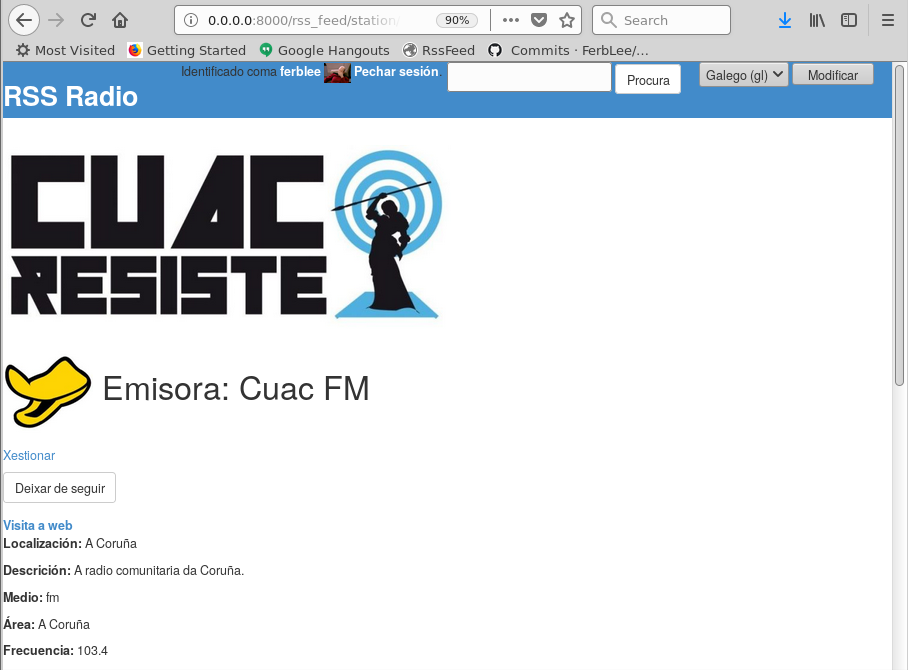
\includegraphics[scale=0.43,keepaspectratio=true]{./images/station_detail_final.png}
	\caption{It8: Vista de detalles de emisora.}
	\label{fig:station_detail_final}
\end{figure}

Novas historias de usuario:
\begin{itemize}
	\item Corrixir internacionalización (Posposto)
	\item Crear \textbf{edición de emisora} e programa.
	\item Implementar \textbf{accións de ouvinte}.
	\item Completar \textbf{vistas de detalle} de emisora e programa
\end{itemize}



\subsection{Iteración 9}

Actualizáronse as vistas de detalle de programa e episodio (ver figura \ref{fig:episode_detail_final}). Implementáronse as accións dos ouvintes: \textbf{Votar os episodios} (Positivo, negativo e desfacer voto), subscribirse, seguir emisora e engadir comentarios.

Ao afrontar a implementación das vistas de edición, discutiuse a cerca da relación entre os usuarios e os seu contido. Chegouse a conclusión de que sería necesaria a creación de \textbf{roles de administración} para programas e emisoras.

Descubríronse unha serie de erros na vista de engadir contidos que foron corrixidos. Non se realizou ningunha actividade no tocante á internacionalización.

\begin{figure}[H]
	\centering
	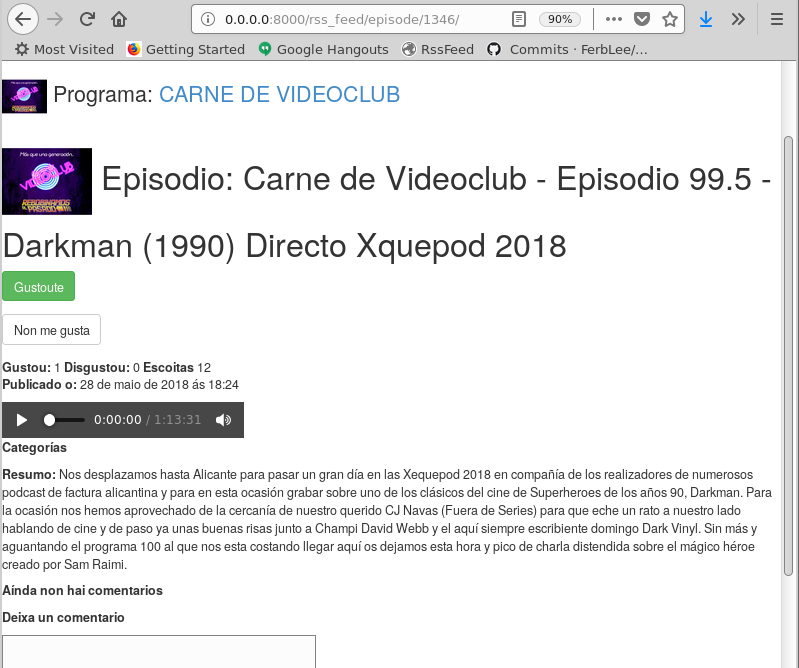
\includegraphics[scale=0.5,keepaspectratio=true]{./images/episode_detail_final.png}
	\caption{It9: Vista de detalles de episodio.}
	\label{fig:episode_detail_final}
\end{figure}

Novas historias de usuario:
\begin{itemize}
	\item Corrixir \textbf{internacionalización}.
	\item Crear \textbf{roles} de usuario.
	\item Crear \textbf{panel de edición} e xestión de emisora e programa.
	\item Implementar as funcións de \textbf{procura} de contidos.
\end{itemize}




\subsection{Iteración 10}

Creáronse os roles de usuario e fíxose o panel de edición e xestión de programas e emisoras (figura \ref{fig:xestionl_final}). A implementación da procura quedou posposta por falta de tempo.

Coméntose a posibilidade de adaptar o estilo da páxina para os dispositivos móbiles.

Novas historias de usuario:
\begin{itemize}
	\item Comezar a redacción da \textbf{documentación}.
	\item Corrixir internacionalización.
	\item Implementar as funcións de procura de contidos.
	\item Adaptar o estilo para \textbf{dispositivos móbiles}.
\end{itemize}

\begin{figure}[h]
	\centering
	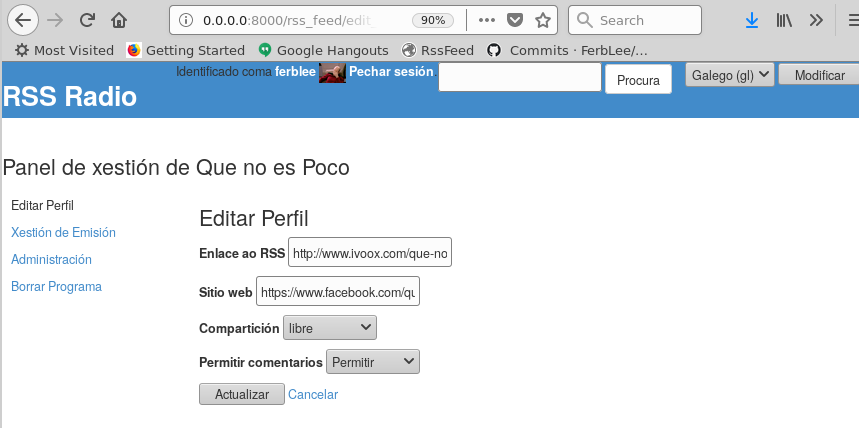
\includegraphics[scale=0.5,keepaspectratio=true]{./images/xestion_final.png}
	\caption{It10: Panel de xestión de programa.}
	\label{fig:xestionl_final}
\end{figure}


\subsection{Iteración 11}


Todos os obxectivos restantes foron cumpridos, sendo o máis destacable a nova vista de \textbf{resultados de busca} (Figura \ref{fig:procura_final}). Implementáronse ferramentas de busca por texto e busca por tag.

A partir de aquí, as sucesivas reunións consistiron en \textbf{revisións desta documentación}. Demos, polo tanto, o desenvolvemento por finalizado.

\begin{figure}[H]
	\centering
	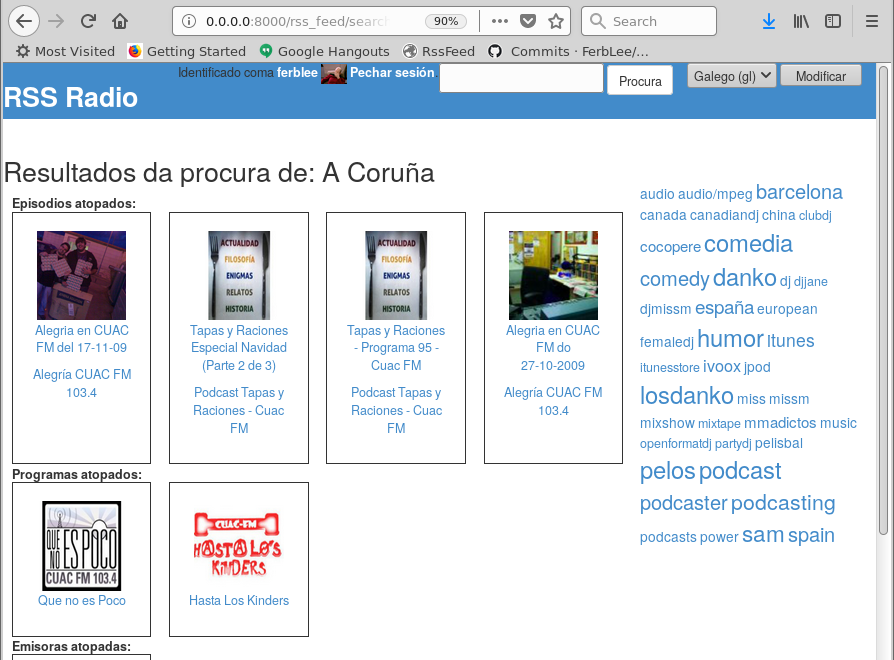
\includegraphics[scale=0.45,keepaspectratio=true]{./images/procura_final.png}
	\caption{It11: Páxina de resultados de busca.}
	\label{fig:procura_final}
\end{figure}


\section{Estudo de custos}

A intención desta sección é facer unha estimación do custo do proxecto. Dado que este foi realizado por unha única persoa levando a cabo distintas tarefas en cada fase do proxecto, estimarase un custe uniforme de 19€/h para todas elas. 

Na táboa \ref{tab:custo} pódese ver o gasto por iteración e o custo total do proxecto.

\begin{table}[h]
	\centering
	\begin{tabular}{|p{5cm}|l|l|}
		\hline
		\rowcolor{blue!10}
		Iteración & Horas de traballo & Custo(€)\\
		\hline
		Primeira reunión & 1 &  19\\
		\hline
		Iteración 1 & 3 &  57\\
		\hline
		Iteración 2 & 12 &  228\\
		\hline
		Iteración 3 & 10 &  190\\
		\hline
		Iteración 4 & 20 &  380\\
		\hline
		Iteración 5 & 25 &  475\\
		\hline
		Iteración 6 & 23 &  437\\
		\hline
		Iteración 7 & 27 &  513\\
		\hline
		Iteración 8 & 32 &  608\\
		\hline
		Iteración 9 & 26 &  494\\
		\hline
		Iteración 10 & 30 &  570\\
		\hline
		Iteración 11 &  18 &  342\\
		\hline
		Escritura da documentación & 45 & 855\\
		\hline
		\textbf{Total} & \textbf{272} & \textbf{5168} \\
		\hline
	\end{tabular}
	\caption{Custo das distintas etapas de traballo.}
\label{tab:custo}
\end{table}


\section{Programación das tarefas}


\begin{figure}[H]
	\centering
	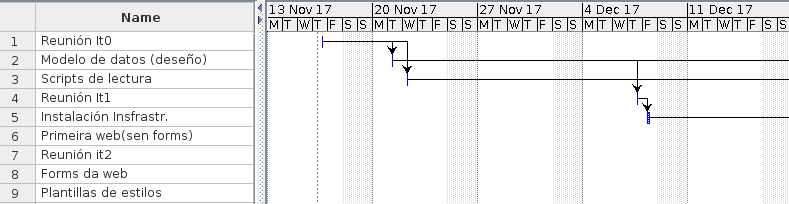
\includegraphics[scale=0.55,keepaspectratio=true]{./images/gantt/gantt1-1.png}
	\caption{Diagrama de Gantt: Novembro 2017 - Decembro.}
	\label{fig:gantt1-1}
\end{figure}

\begin{figure}[H]
	\centering
	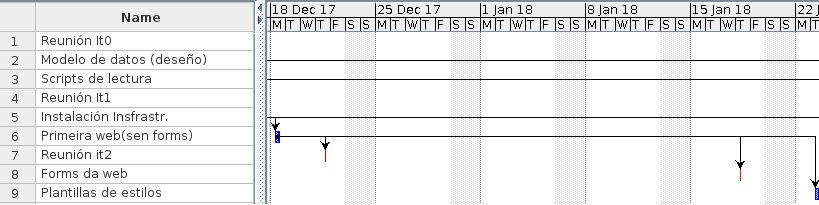
\includegraphics[scale=0.5,keepaspectratio=true]{./images/gantt/gantt1-2.png}
	\caption{Diagrama de Gantt: Decembro 2017 - Xaneiro 2018.}
	\label{fig:gantt1-2}
\end{figure}

\begin{figure}[H]
	\centering
	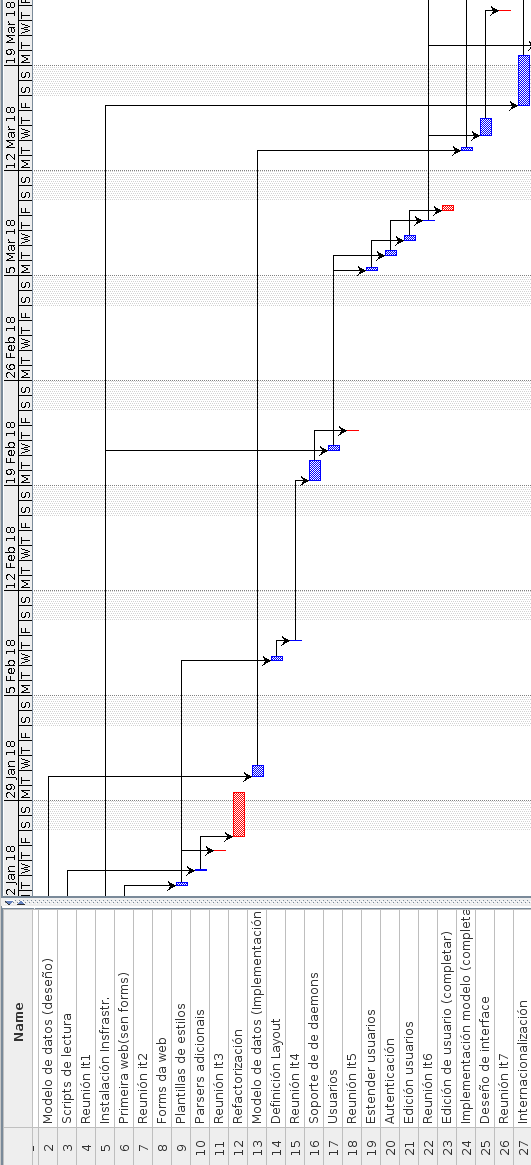
\includegraphics[scale=0.5,keepaspectratio=true]{./images/gantt/gantt2.png}
	\caption{Diagrama de Gantt: Xaneiro 2018 - Marzo 2018. }
	\label{fig:gantt2}
\end{figure}

\begin{figure}[H]
	\centering
	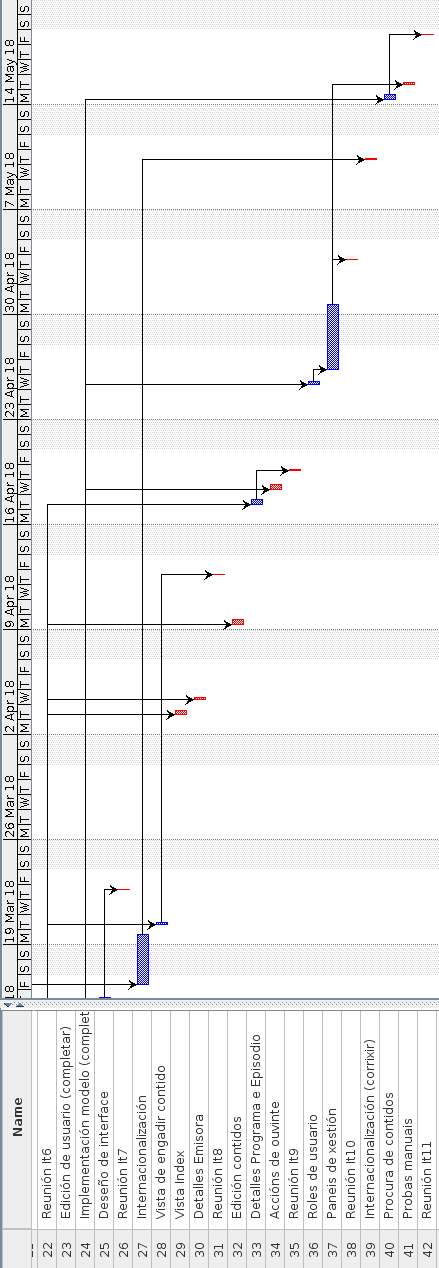
\includegraphics[scale=0.4,keepaspectratio=true]{./images/gantt/gantt3.png}
	\caption{Diagrama de Gantt: Marzo 2018 - Maio 2018. }
	\label{fig:gantt3}
\end{figure}

\begin{figure}[H]
	\centering
	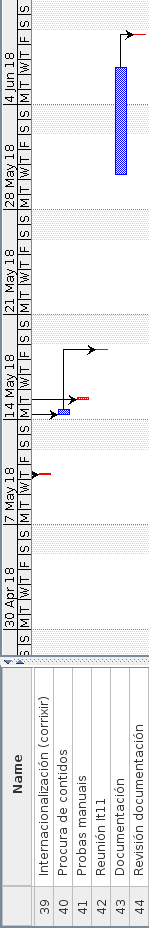
\includegraphics[scale=0.6,keepaspectratio=true]{./images/gantt/gantt4.png}
	\caption{Diagrama de Gantt: Maio 2018 - Xuño 2018. }
	\label{fig:gantt4}
\end{figure}